\chapter{Related Work}
In this chapter we describe prior work in the area of finding optimal join order.

\section{TreeOpt Algorithm}
Some of the earliest work on finding optimal join order was done by Ibraraki and Kameda\cite{ibaraki1984optimal}.  They describes an algorithm for finding the optimal nesting order for tree queries ie: queries whose join graphs form a tree for nested loop join. Finding a solution for general graphs is NP-Hard, however for this special case it is possible to find the optimal solution in polynomial time. \\

A cost function f is said to satisfy the \textit{adjacent sequence interchange} property (ASI property in short) if there exists a rank function $r_{f}$ such that $f(AS_{1}S_{2}B) <= f(AS_{1}S_{2}B)$ if and only if $r_{f}(S_{1}) <= r_{f}(S_{2})$. It is known that if a cost function $f$ satisfies the ASI property, an optimal sequence can be found in $O(n log(n))$ where the order constraints are series parallel. In our case, the order constraints are directed tree which is a special case of series parallel constraints. \\

Refer to Algorithm \ref{alg:treeopt}. Set one of the nodes in tree as root R, call \textsc{TreeOpt} $(T,R)$. Every node in the tree has a rank given by rank function $r_{f}$. Until we reduce the tree to a chain, find a wedge in the tree and reduce it a chain where the nodes are listed in the order of their rank. However there might be ordering constraints within in a chain. The subroutine \textsc{Normalize} in called on each chain prior to reduction which combines nodes $S_{i}$ and $S{j}$ in the chain if $r_{f}(S_{i}) > r_{f}(S_{j})$ and $S_{i}$ occurs before $S_{j}$, a new label $S_{k}$ is assigned for combined entity containing $S_{i} \cup S_{j}$ and its rank is recalculated.  \\

\textsc{TreeOpt} is called n times, each time with different node as root. In the end we have an optimal tree for each node as root. The tree with the lowest cost among these is  indeed the optimal tree. Complexity : $O(n^2 log(n))$.

\begin{algorithm}
  \caption{Finding Optimal Nesting Order for Tree Queries
    \label{alg:treeopt}}
	\begin{algorithmic}[1]
	\Function{TreeOpt}{$T,R$}
		\State $rt \gets$ directed tree rooted at R   
		\While {$rt$ is not a chain}
			\State Find a wedge in the tree $rt$
			\State Apply \textsc{Normalize} to each chain of the wedge.
			\State Merge the two chains into one by ordering the nodes by their ranks.		
		\EndWhile
	\EndFunction
  \end{algorithmic}
\end{algorithm}

For optimizing cyclic join graphs the strategy is to first transform the graph into an acyclic join graph before running \textsc{TreeOpt}. This acyclic join graph needs to chosen with care. Note that when ordering the nodes, the goal was to reduce the number of page fetches. This in nested loop join means keeping size of intermediary relation low. Hence one good candidate for the tree is Minimum Spanning Tree with edge weights as $|R_{i}||R_{j}| \sigma_{R_{i}R_{j}}$. However it is shown experimentally that this method is not reliable.

\section{Heuristic for Cyclic Queries}
\textsc{TreeOpt} generates optimal plan for any acyclic join graph in polynomial time. However for cyclic queries, it does a bad job at even producing a near optimal plan. Raghavan et al. \cite{raghavan2009multi} propose a new algorithm called FAB (Forward and Backward) algorithm for producing better plans for cyclic join graph in polynomial time. \\

FAB approach uses a global-impact based ordering, in which the global impact of each relation explored and used to decide the ordering. The global impact of a  relation $R_{i}$ is the product of the size of all other relations and join selectivity not related to $R_{i}$. Intuitively if node $R_{i}$ has least impact, it means that it itself has a combination of large size and low join selectivity. The FAB algorithm picks the node with least impact and puts it as the last node to be joined. It then recalculates the impact of each node after removing the element from the join graph. \\

This approach works quite well for cyclic join graphs but note it not guaranteed to produce optimal plan always. The paper proposes a query aware approach where given a query, we try to infer if the join graph is linear, acyclic or cyclic. For the first two, use the TreeOpt algorithm and for third use FAB. \\

Note that FAB and TreeOpt are both used to generate left deep join trees. They do not help in any way to find the optimal solution in the space of all bushy join trees. 

\section{DP and Memoization based join enumeration}
Two approaches have done well at exploring and finding the optimal plan in the space of all bushy join orderings : bottom-up join enumeration via dynamic programming and top-down join enumeration via memoization. Moerkotte and Neumann \cite{moerkotte2006analysis} presented an efficient dynamic programming based algorithm (\textsc{DPccp}). DeHaan and Tompa \cite{dehaan2007optimal} proposed an efficient top-down algorithm (\textsc{TDMinCutLazy}). Fender and Moerkotte \cite{fender2011new} proposed an alternative top-down join enumeration strategy (\textsc{TDMinCutBranch}), which is almost as efficient as \textsc{DPccp}. In the following year, Fender et al.\cite{fender2012effective} proposed another top-down enumeration strategy \textsc{TDMinCutConservative} which is currently the best.

\subsection{Generic Top-Down Enumeration}
Top-Down join enumeration has a clear advantage over Bottom-Up style as it enables pruning. We describe a generic top-down enumeration via \textsc{TDPlanGen} (see pseudocode in Figure \ref{fig:tdplangen}). Like in dynamic programming, TDPlanGen initializes the building blocks for atomic relations first (line 2). In line 3, the subroutine \textsc{TDPGSub} is called, which traverses recursively through the search space. At each invocation of \textsc{TDPGSub}, a connected subgraph $G_{|S}$ is given. If the best tree for this graph is not known, a suitable partitioning strategy is used to partition $S$ into two sets $S_{1}$ and $S_{2}$ such that the following condition are satisfied :
\begin{itemize}
	\item $S_{1}$ with $S_{1} \subset S$ induces a connected subgraph $G_{|S_{1}}$
	\item $S_{2}$ with $S_{2} \subset S$ induces a connected subgraph $G_{|S_{2}}$
	\item $S_{1} \cup S_{2} = S$ and $S_{1} \cap S_{2} = \phi$
	\item $\exists (v_{1}, v_{2}) \in E$ | $v_{1} \in S_{1} \wedge v_{2} \in S_{2}$
\end{itemize}
If $(S_{1},S_{2})$ is valid, so is $(S_{2},S_{1})$. The set of all pairs $(S_{1},S_{2})$ such that symmetric pairs are counted only once is denoted by $P^{sym}_{ccp}(S)$. A subroutine \textsc{BuildTree} is called which recursively calls \textsc{TDPGSub} on subgraph induced by $S_{1}$ and subgraph induced by $S_{2}$. The recursive decent stops when $|S| = 1$ or the best tree is already known. Once all the possibilities have been tried. \textsc{BuildTree} updates memotable $BestTree$ if a plan better than existing plan is found. After all $(S_{1}, S_{2}) \in P^{sym}_{ccp}(S)$ have been tried, the entry in $BestTree[S]$ corresponds the optimal join tree for set of relations in $S$.

\begin{figure}[here]
\begin{center}
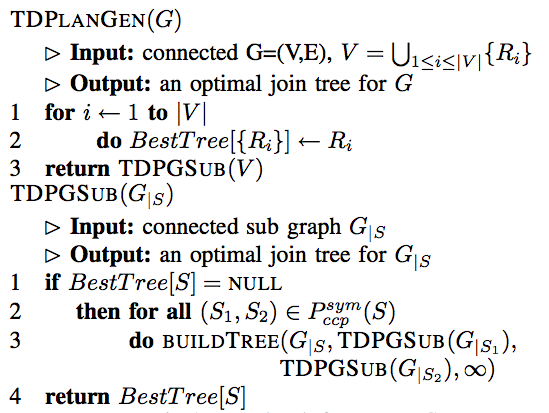
\includegraphics[width=9cm]{Figures/tdplangen.png}
\end{center}
\caption{Pseudocode for TDPLANGEN}
\label{fig:tdplangen}
\end{figure}

Depending on the choice of partitioning algorithm, the overall performance of \textsc{TDPlanGen} can vary by orders of magnitude. Since \textsc{TDPlanGen} is top-down  we can easily apply existing pruning techniques to prevent exploration of entire sub-trees. Later in section \ref{conservativePartitioning} we describe the \textsc{MinCutConservative} partitioning algorithm and how we can use it in transformational setting. 